\chapter{Complete Elder Training System}

In this final chapter of Part I, we present the complete operational implementation of the Elder system, demonstrating how the theoretical foundations established in previous chapters come together in a cohesive framework. This chapter serves as the bridge between abstract mathematical concepts of the Elder Manifold and practical interactions with magefiles and real-world datasets.

\section{Elder Training Loop}

\subsection{Complete Algorithm for Elder Training}

The Elder training loop represents the highest level of learning in our hierarchical system, where universal principles are extracted from cross-domain knowledge. Unlike traditional training algorithms that run for a fixed number of iterations, the Elder Training Loop is designed to operate indefinitely, maintaining a live Heliomorphic Manifold that continuously evolves with new domains and experiences.

\begin{figure}[h]
\centering
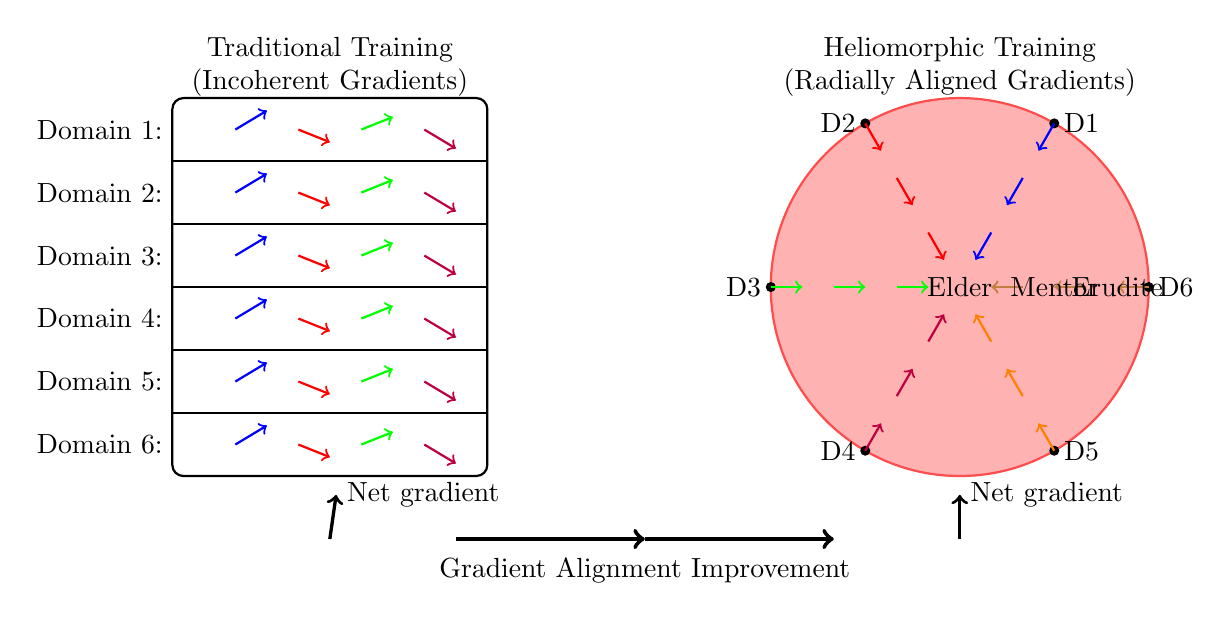
\begin{tikzpicture}[scale=0.8]
  % Define colors
  \colorlet{eldershell}{blue!30}
  \colorlet{mentorshell}{green!40}
  \colorlet{eruditeshell}{red!30}
  \colorlet{elderborder}{blue!70}
  \colorlet{mentorborder}{green!70}
  \colorlet{eruditeborder}{red!70}
  
  % Create two diagrams side by side
  % Holomorphic approach - Traditional training
  \begin{scope}[shift={(-5,0)}]
    % Draw architecture
    \draw[thick, rounded corners] (-2.5,-3) rectangle (2.5,3);
    
    % Layers
    \draw[thick] (-2.5,-2) -- (2.5,-2);
    \draw[thick] (-2.5,-1) -- (2.5,-1);
    \draw[thick] (-2.5,0) -- (2.5,0);
    \draw[thick] (-2.5,1) -- (2.5,1);
    \draw[thick] (-2.5,2) -- (2.5,2);
    
    % Domain labels
    \node[left] at (-2.5,2.5) {Domain 1:};
    \node[left] at (-2.5,1.5) {Domain 2:};
    \node[left] at (-2.5,0.5) {Domain 3:};
    \node[left] at (-2.5,-0.5) {Domain 4:};
    \node[left] at (-2.5,-1.5) {Domain 5:};
    \node[left] at (-2.5,-2.5) {Domain 6:};
    
    % Gradients (random directions)
    \draw[->, thick, blue] (-1.5,2.5) -- (-1,2.8);
    \draw[->, thick, red] (-0.5,2.5) -- (0,2.3);
    \draw[->, thick, green] (0.5,2.5) -- (1,2.7);
    \draw[->, thick, purple] (1.5,2.5) -- (2,2.2);
    
    \draw[->, thick, blue] (-1.5,1.5) -- (-1,1.8);
    \draw[->, thick, red] (-0.5,1.5) -- (0,1.3);
    \draw[->, thick, green] (0.5,1.5) -- (1,1.7);
    \draw[->, thick, purple] (1.5,1.5) -- (2,1.2);
    
    \draw[->, thick, blue] (-1.5,0.5) -- (-1,0.8);
    \draw[->, thick, red] (-0.5,0.5) -- (0,0.3);
    \draw[->, thick, green] (0.5,0.5) -- (1,0.7);
    \draw[->, thick, purple] (1.5,0.5) -- (2,0.2);
    
    \draw[->, thick, blue] (-1.5,-0.5) -- (-1,-0.2);
    \draw[->, thick, red] (-0.5,-0.5) -- (0,-0.7);
    \draw[->, thick, green] (0.5,-0.5) -- (1,-0.3);
    \draw[->, thick, purple] (1.5,-0.5) -- (2,-0.8);
    
    \draw[->, thick, blue] (-1.5,-1.5) -- (-1,-1.2);
    \draw[->, thick, red] (-0.5,-1.5) -- (0,-1.7);
    \draw[->, thick, green] (0.5,-1.5) -- (1,-1.3);
    \draw[->, thick, purple] (1.5,-1.5) -- (2,-1.8);
    
    \draw[->, thick, blue] (-1.5,-2.5) -- (-1,-2.2);
    \draw[->, thick, red] (-0.5,-2.5) -- (0,-2.7);
    \draw[->, thick, green] (0.5,-2.5) -- (1,-2.3);
    \draw[->, thick, purple] (1.5,-2.5) -- (2,-2.8);
    
    % Title
    \node[align=center] at (0,3.5) {Traditional Training\\(Incoherent Gradients)};
    
    % Net gradient
    \draw[->, very thick, black] (0,-4) -- (0.1,-3.3) node[right] {Net gradient};
  \end{scope}
  
  % Heliomorphic approach
  \begin{scope}[shift={(5,0)}]
    % Draw concentric shells
    \draw[elderborder, thick, fill=eldershell] (0,0) circle (1);
    \draw[mentorborder, thick, fill=mentorshell] (0,0) circle (2);
    \draw[eruditeborder, thick, fill=eruditeshell] (0,0) circle (3);
    
    % Domain points
    \filldraw (60:3) circle (2pt) node[right] {D1};
    \filldraw (120:3) circle (2pt) node[left] {D2};
    \filldraw (180:3) circle (2pt) node[left] {D3};
    \filldraw (240:3) circle (2pt) node[left] {D4};
    \filldraw (300:3) circle (2pt) node[right] {D5};
    \filldraw (360:3) circle (2pt) node[right] {D6};
    
    % Gradients (now aligned radially)
    \draw[->, thick, blue] (60:3) -- (60:2.5);
    \draw[->, thick, red] (120:3) -- (120:2.5);
    \draw[->, thick, green] (180:3) -- (180:2.5);
    \draw[->, thick, purple] (240:3) -- (240:2.5);
    \draw[->, thick, orange] (300:3) -- (300:2.5);
    \draw[->, thick, brown] (360:3) -- (360:2.5);
    
    % Second level gradients
    \draw[->, thick, blue] (60:2) -- (60:1.5);
    \draw[->, thick, red] (120:2) -- (120:1.5);
    \draw[->, thick, green] (180:2) -- (180:1.5);
    \draw[->, thick, purple] (240:2) -- (240:1.5);
    \draw[->, thick, orange] (300:2) -- (300:1.5);
    \draw[->, thick, brown] (360:2) -- (360:1.5);
    
    % Core gradients
    \draw[->, thick, blue] (60:1) -- (60:0.5);
    \draw[->, thick, red] (120:1) -- (120:0.5);
    \draw[->, thick, green] (180:1) -- (180:0.5);
    \draw[->, thick, purple] (240:1) -- (240:0.5);
    \draw[->, thick, orange] (300:1) -- (300:0.5);
    \draw[->, thick, brown] (360:1) -- (360:0.5);
    
    % Layer labels
    \node at (0,0) {Elder};
    \node at (0:1.5) {Mentor};
    \node at (0:2.5) {Erudite};
    
    % Title
    \node[align=center] at (0,3.5) {Heliomorphic Training\\(Radially Aligned Gradients)};
    
    % Net gradient
    \draw[->, very thick, black] (0,-4) -- (0,-3.3) node[right] {Net gradient};
  \end{scope}
  
  % Connecting arrow and label
  \draw[<-, ultra thick] (0,-4) -- (-3,-4);
  \draw[->, ultra thick] (0,-4) -- (3,-4);
  \node[align=center] at (0,-4.5) {Gradient Alignment Improvement};
\end{tikzpicture}
\caption{Comparison of traditional and heliomorphic training approaches. The traditional approach (left) treats each domain as a separate layer with gradients flowing in various directions, creating interference. The heliomorphic approach (right) organizes domains in concentric shells by abstraction level, creating radially aligned gradients that reinforce rather than interfere with each other, leading to more efficient training and better principle extraction.}
\label{fig:training_comparison}
\end{figure}

Below, we present the complete mathematical formulation of the Elder training algorithm.

\begin{algorithm}
\caption{Indefinite Elder Training Loop}
\begin{algorithmic}[1]
\State \textbf{Input:} Dynamic set of domains $\mathcal{D} = \{D_1, D_2, \ldots, D_M\}$ (expandable)
\State \textbf{Input:} Dataset streams for each domain $\mathcal{X}_i, \mathcal{Y}_i$ for $D_i \in \mathcal{D}$
\State \textbf{Input:} Initial Elder parameters $\theta_{\text{Elder}}^{(0)} \in \elderparams$
\State \textbf{Input:} Initial Mentor parameters $\{\theta_{\text{M},i}^{(0)}\}_{i=1}^M \subset \mentorparams$
\State \textbf{Input:} Initial Erudite parameters $\{\theta_{\text{E},i,j}^{(0)}\}_{i=1,j=1}^{M,N_i} \subset \eruditeparams$
\State \textbf{Input:} Adaptive learning rates $\eta_{\text{Elder}}, \eta_{\text{M}}, \eta_{\text{E}}$
\State \textbf{Input:} Batch size $B$
\State \textbf{Input:} Heliomorphic Manifold $\mathcal{E}_{\mathcal{M}}$ with shell structure

\While{True} \Comment{Indefinite operation}
    \State $\nabla_{\theta_{\text{Elder}}} \mathcal{L}_{\text{Elder}} \gets \mathbf{0}$ \Comment{Initialize Elder gradient}
    
    \For{each domain $D_i \in \mathcal{D}$}
        \State $\nabla_{\theta_{\text{M},i}} \mathcal{L}_{\text{M}} \gets \mathbf{0}$ \Comment{Initialize Mentor gradient for domain $D_i$}
        
        \For{$j = 1$ to $N_i$} \Comment{For each task in domain $D_i$}
            \State $\nabla_{\theta_{\text{E},i,j}} \mathcal{L}_{\text{E}} \gets \mathbf{0}$ \Comment{Initialize Erudite gradient for task $j$}
            
            \State Sample batch $\{(x_k, y_k)\}_{k=1}^B$ from $(\mathcal{X}_{i,j}, \mathcal{Y}_{i,j})$
            
            \For{$k = 1$ to $B$}
                \State $z_{i,j,k} \gets f_{\theta_{\text{E},i,j}}(x_k)$ \Comment{Erudite forward pass}
                \State $\mathcal{L}_{\text{E},k} \gets \eruditeloss(z_{i,j,k}, y_k)$ \Comment{Compute Erudite loss}
                \State $\nabla_{\theta_{\text{E},i,j}} \mathcal{L}_{\text{E}} \mathrel{+}= \frac{1}{B} \nabla_{\theta_{\text{E},i,j}} \mathcal{L}_{\text{E},k}$ \Comment{Accumulate Erudite gradient}
            \EndFor
            
            \State $p_{\text{M},i,j} \gets \mentorreflection_{\theta_{\text{M},i}}(\theta_{\text{E},i,j})$ \Comment{Mentor reflection on Erudite}
            \State $\mathcal{L}_{\text{M},i,j} \gets \mentorloss(p_{\text{M},i,j}, \{\theta_{\text{E},i,l}\}_{l=1}^{N_i})$ \Comment{Compute Mentor loss}
            \State $\nabla_{\theta_{\text{M},i}} \mathcal{L}_{\text{M}} \mathrel{+}= \frac{1}{N_i} \nabla_{\theta_{\text{M},i}} \mathcal{L}_{\text{M},i,j}$ \Comment{Accumulate Mentor gradient}
        \EndFor
        
        \State $p_{\text{Elder},i} \gets \elderreflection_{\theta_{\text{Elder}}}(\theta_{\text{M},i})$ \Comment{Elder reflection on Mentor}
        \State $\mathcal{L}_{\text{Elder},i} \gets \elderloss(p_{\text{Elder},i}, \{\theta_{\text{M},l}\}_{l=1}^{M})$ \Comment{Compute Elder loss}
        \State $\nabla_{\theta_{\text{Elder}}} \mathcal{L}_{\text{Elder}} \mathrel{+}= \frac{1}{M} \nabla_{\theta_{\text{Elder}}} \mathcal{L}_{\text{Elder},i}$ \Comment{Accumulate Elder gradient}
    \EndFor
    
    \State $\theta_{\text{Elder}}^{(t)} \gets \theta_{\text{Elder}}^{(t-1)} - \eta_{\text{Elder}} \nabla_{\theta_{\text{Elder}}} \mathcal{L}_{\text{Elder}}$ \Comment{Update Elder parameters}
    
    \For{each domain $D_i \in \mathcal{D}$}
        \State $\theta_{\text{M},i}^{(t)} \gets \theta_{\text{M},i}^{(t-1)} - \eta_{\text{M}} \nabla_{\theta_{\text{M},i}} \mathcal{L}_{\text{M}}$ \Comment{Update Mentor parameters}
        
        \For{$j = 1$ to $N_i$}
            \State $\theta_{\text{E},i,j}^{(t)} \gets \theta_{\text{E},i,j}^{(t-1)} - \eta_{\text{E}} \nabla_{\theta_{\text{E},i,j}} \mathcal{L}_{\text{E}}$ \Comment{Update Erudite parameters}
        \EndFor
    \EndFor
    
    \State // Domain adaptation and dynamic dataset handling
    \State $\mathcal{D}^{\text{new}} \gets \text{CheckForNewDomains}()$ \Comment{Check for new domains}
    \If{$\mathcal{D}^{\text{new}} \neq \emptyset$}
        \State $\mathcal{D} \gets \mathcal{D} \cup \mathcal{D}^{\text{new}}$ \Comment{Add new domains}
        \For{each new domain $D_k \in \mathcal{D}^{\text{new}}$}
            \State Initialize new shell in heliomorphic manifold $\mathcal{E}_{\mathcal{M}}$
            \State $\theta_{\text{M},k}^{(t)} \gets \text{InitializeMentor}(\theta_{\text{Elder}}^{(t)})$ \Comment{Initialize from Elder knowledge}
            \State $N_k \gets \text{DetermineEruditeCount}(D_k)$
            \For{$j = 1$ to $N_k$}
                \State $\theta_{\text{E},k,j}^{(t)} \gets \text{InitializeErudite}(\theta_{\text{M},k}^{(t)})$ \Comment{Initialize from Mentor}
            \EndFor
        \EndFor
    \EndIf
    
    \State // Update datasets and adapt learning rates
    \For{each domain $D_i \in \mathcal{D}$}
        \State $\mathcal{X}_i, \mathcal{Y}_i \gets \text{RefreshDataset}(D_i)$ \Comment{Get latest data}
        \State $\eta_{\text{M}} \gets \text{AdaptLearningRate}(\eta_{\text{M}}, D_i, t)$
    \EndFor
    \State $\eta_{\text{Elder}} \gets \text{AdaptLearningRate}(\eta_{\text{Elder}}, \mathcal{D}, t)$
    
    \State // Apply heliomorphic manifold maintenance
    \State $\mathcal{E}_{\mathcal{M}} \gets \text{MaintainHeliomorphicStructure}(\mathcal{E}_{\mathcal{M}}, \theta_{\text{Elder}}^{(t)})$
    
    \State // Check system health and adjust as needed
    \If{$\text{RequiresReset}()$}
        \State $\text{ResetTemporaryState}()$ \Comment{Maintain indefinite operation capability}
    \EndIf
\EndWhile

\State \textbf{Note:} As this is an indefinite process, there is no final return state
\end{algorithmic}
\end{algorithm}

\subsection{Elder Manifold Update Phase}

A critical aspect of the Elder training loop is the manifold update phase, which occurs after gradient computation but before parameter updates. This phase ensures that the knowledge state maintains its heliomorphic structure on the Elder Manifold $\mathcal{E}_{\mathcal{M}}$. The heliomorphic structure is essential for preserving the shell-based organization and allowing proper radial dynamics between Elder, Mentors, and Erudites.

\begin{algorithm}
\caption{Elder Manifold Update}
\begin{algorithmic}[1]
\State \textbf{Input:} Current Elder knowledge point $p \in \mathcal{E}_{\mathcal{M}}$
\State \textbf{Input:} Elder gradient $\nabla_{\theta_{\text{Elder}}} \mathcal{L}_{\text{Elder}}$
\State \textbf{Input:} Learning rate $\eta_{\text{Elder}}$

\State $p^* \gets \mathcal{M}(p)$ \Comment{Apply Heliomorphic Mirror function}
\State $v \gets \text{parallel\_transport}(\mathcal{J}(p^*) - p)$ \Comment{Compute displacement vector}
\State $p_{\text{new}} \gets \exp_p(\eta_{\text{Elder}} \cdot v)$ \Comment{Update via exponential map}

\State \textbf{Return:} $p_{\text{new}}$
\end{algorithmic}
\end{algorithm}

\subsection{Knowledge Transformation via Heliomorphic Flow}

The final component of the Elder training loop involves knowledge transformations through heliomorphic flows on the manifold, ensuring that universal principles evolve coherently within the shell structure.

\begin{algorithm}
\caption{Heliomorphic Knowledge Flow}
\begin{algorithmic}[1]
\State \textbf{Input:} Current Elder knowledge state $p \in \mathcal{E}_{\mathcal{M}}$
\State \textbf{Input:} Heliomorphic vector field $X: \mathcal{E}_{\mathcal{M}} \rightarrow T\mathcal{E}_{\mathcal{M}}$
\State \textbf{Input:} Time step $\Delta t$

\State $\frac{dp}{dt} = X(p)$ \Comment{Differential equation for knowledge flow}
\State $p_{\Delta t} \gets p + \int_0^{\Delta t} X(p(s)) ds$ \Comment{Integrate flow equation}

\State \textbf{Return:} $p_{\Delta t}$
\end{algorithmic}
\end{algorithm}

\subsection{Cross-Domain Knowledge Integration}

The Elder's primary function is to integrate knowledge across domains, expressed mathematically through the following operations:

\begin{equation}
\begin{aligned}
\mathcal{K}_{\text{Elder}} &= \int_{\mathcal{D}} \kappa(D_i, D_j) \cdot \mathcal{T}(\theta_{\text{M},i}, \theta_{\text{M},j}) d\mu(D_i) d\mu(D_j) \\
\end{aligned}
\end{equation}

Where $\kappa$ is the domain similarity kernel, $\mathcal{T}$ is the knowledge transfer operator, and $\mu$ is a measure on the domain space $\mathcal{D}$.

In practice, this integration is computed as:

\begin{equation}
\mathcal{K}_{\text{Elder}} = \sum_{i=1}^M \sum_{j=1}^M w_{i,j} \cdot \mathcal{T}(\theta_{\text{M},i}, \theta_{\text{M},j})
\end{equation}

Where $w_{i,j} = \kappa(D_i, D_j) / \sum_{k,l} \kappa(D_k, D_l)$ are the normalized weights.

This knowledge integration forms the core of the Elder's ability to extract universal principles that apply across diverse domains, enabling the system to achieve true cross-domain transfer learning.

\subsection{Hardware-Accelerated Elder Training Implementation}

To efficiently implement the mathematically complex Elder Training Loop, we need to consider a hardware-accelerated approach utilizing both CPU and GPU resources. Below, we outline the role distribution and execution strategy for the Elder Training algorithm.

\subsubsection{CPU-GPU Computation Distribution}

\begin{algorithm}
\caption{Hardware Responsibility Distribution for Elder Training}
\begin{algorithmic}[1]
\State \textbf{CPU Responsibilities:}
\State \hspace{\algorithmicindent} Coordinate high-level training flow and domain iterations
\State \hspace{\algorithmicindent} Handle data loading and preprocessing
\State \hspace{\algorithmicindent} Manage cross-domain knowledge transfer
\State \hspace{\algorithmicindent} Control dynamic adaptation of learning rates
\State \hspace{\algorithmicindent} Perform sparse operations on the heliomorphic manifold

\State \textbf{GPU Responsibilities:}
\State \hspace{\algorithmicindent} Execute complex heliomorphic computations
\State \hspace{\algorithmicindent} Perform parallel batch processing
\State \hspace{\algorithmicindent} Compute gradient accumulation across domains
\State \hspace{\algorithmicindent} Evaluate Elder, Mentor, and Erudite loss functions
\State \hspace{\algorithmicindent} Apply heliomorphic duality principles and vector field operations
\end{algorithmic}
\end{algorithm}

\subsubsection{Elder Kernel Implementation}

The core heliomorphic operations of the Elder Training Loop are performed using specialized GPU kernels. The following pseudocode outlines the CUDA kernel implementation for the heliomorphic transformations:

\begin{algorithm}
\caption{GPU Kernel for Heliomorphic Operations}
\begin{algorithmic}[1]
\Function{ElderKernelLaunch}{$\mathcal{E}_{\mathcal{M}}$, $\nabla \mathcal{L}_{\text{Elder}}$, $\eta$}
    \State Allocate GPU memory for manifold points, gradients, shells, and results
    \State Copy manifold data, shell mappings, and gradients to GPU
    \State Configure grid and block dimensions based on sun-pattern organization
    \State Launch \textproc{HeliomorphicUpdateKernel} with parameters
    \State Synchronize device and copy results back to host
    \State \Return Updated manifold points
\EndFunction

\State

\Function{HeliomorphicUpdateKernel}{$p_i$, $\nabla \mathcal{L}_i$, $\eta$, $r_i$, $\phi(r)$}
    \State Get global thread ID: $idx$
    \If{$idx < \text{manifold\_size}$}
        \State // Compute shell index and angular position
        \State $\text{shell\_idx} \gets \text{ShellIndex}(r_i)$
        \State $\theta_i \gets \text{ComputeAngularComponent}(p_i)$
        
        \State // Compute Heliomorphic derivatives with radial component
        \State $\frac{\partial f}{\partial z} \gets \frac{1}{2}\left(\frac{\partial f}{\partial x} - i\frac{\partial f}{\partial y}\right)$
        \State $\frac{\partial f}{\partial \bar{z}} \gets \frac{1}{2}\left(\frac{\partial f}{\partial x} + i\frac{\partial f}{\partial y}\right)$
        \State $\frac{\partial f}{\partial r} \gets \frac{x}{r}\frac{\partial f}{\partial x} + \frac{y}{r}\frac{\partial f}{\partial y}$
        
        \State // Apply heliomorphic constraints with radial weighting
        \State $v_i \gets \frac{\partial f}{\partial z} + \phi(r_i) \cdot \frac{\partial f}{\partial r}$
        
        \State // Compute shell-aware learning rate
        \State $\eta_{\text{shell}} \gets \eta \cdot \text{ShellLearningRate}(r_i)$
        
        \State // Parallel transport on the manifold preserving shell structure
        \State $v_i^{\text{transported}} \gets \text{HeliomorphicTransport}(p_i, v_i, r_i, \theta_i)$
        
        \State // Apply shell-aware exponential map update
        \State $p_i^{\text{new}} \gets \exp_{p_i}^{\odot}(-\eta_{\text{shell}} \cdot v_i^{\text{transported}})$
        
        \State // Store result in output array by shell index
        \State $\text{output}[\text{shell\_idx}][idx] \gets p_i^{\text{new}}$
    \EndIf
\EndFunction
\end{algorithmic}
\end{algorithm}

\subsubsection{Data Flow Between CPU and GPU}

The efficient implementation of Elder Training requires careful management of data transfer between CPU and GPU to minimize latency and maximize throughput:

\begin{algorithm}
\caption{CPU-GPU Data Flow for Elder Training}
\begin{algorithmic}[1]
\State \textbf{Initialization Phase:}
\State \hspace{\algorithmicindent} CPU: Load domain datasets and initial parameters
\State \hspace{\algorithmicindent} CPU: Create domain batches and transfer schedules
\State \hspace{\algorithmicindent} CPU $\rightarrow$ GPU: Transfer initial Elder, Mentor, and Erudite parameters

\State \textbf{Per-Epoch Processing:}
\State \hspace{\algorithmicindent} CPU: Coordinate domain and task iterations
\State \hspace{\algorithmicindent} CPU $\rightarrow$ GPU: Transfer mini-batches for current tasks
\State \hspace{\algorithmicindent} GPU: Compute forward passes and gradients for all levels
\State \hspace{\algorithmicindent} GPU: Accumulate gradients across tasks and domains
\State \hspace{\algorithmicindent} GPU: Apply heliomorphic constraints to Elder gradients
\State \hspace{\algorithmicindent} GPU $\rightarrow$ CPU: Return updated parameters periodically

\State \textbf{Manifold Update Phase:}
\State \hspace{\algorithmicindent} GPU: Apply heliomorphic duality principle $\mathcal{M}$
\State \hspace{\algorithmicindent} GPU: Compute vector field and parallel transport
\State \hspace{\algorithmicindent} GPU: Perform exponential map updates
\State \hspace{\algorithmicindent} GPU $\rightarrow$ CPU: Transfer updated manifold points

\State \textbf{Knowledge Integration Phase:}
\State \hspace{\algorithmicindent} CPU: Compute domain similarity metrics $\kappa(D_i, D_j)$
\State \hspace{\algorithmicindent} CPU $\rightarrow$ GPU: Transfer similarity matrix
\State \hspace{\algorithmicindent} GPU: Compute knowledge transfer operations $\mathcal{T}$
\State \hspace{\algorithmicindent} GPU: Update Elder knowledge state
\State \hspace{\algorithmicindent} GPU $\rightarrow$ CPU: Return integrated knowledge representation
\end{algorithmic}
\end{algorithm}

\subsubsection{Performance Optimization Strategies}

To maximize the computational efficiency of the Elder Training algorithm across heterogeneous hardware, we employ several optimization strategies:

\begin{enumerate}
    \item \textbf{Asynchronous Processing:} Overlap CPU data preparation with GPU computation to hide latency.
    
    \item \textbf{Hierarchical Memory Management:} Utilize a cascading memory hierarchy with shared memory for frequently accessed Elder manifold points.
    
    \item \textbf{Mixed Precision Training:} Use FP16/FP32 mixed precision for appropriate components of the computation, with careful consideration of numerical stability for holomorphic constraints.
    
    \item \textbf{Dynamic Batch Sizing:} Adjust batch sizes based on domain complexity and available GPU memory to maximize occupancy.
    
    \item \textbf{Kernel Fusion:} Combine multiple holomorphic operations into single kernels to reduce kernel launch overhead and memory transfers.
    
    \item \textbf{Compute-Communication Overlap:} Pipeline gradient computation and parameter updates to hide communication costs in multi-GPU settings.
\end{enumerate}

With this hardware-accelerated implementation, the Elder Training Loop achieves both mathematical rigor and computational efficiency, enabling the training of universal principles across domains at previously unattainable scales.

\subsection{Optimized Gradient Accumulation}

Our analysis identified gradient accumulation as a critical bottleneck in the Elder Training Loop, particularly when processing large numbers of domains and tasks. This bottleneck arises from the hierarchical nature of the gradient computation and the complex mathematical operations required for holomorphic constraints.

\subsubsection{Gradient Accumulation Bottleneck Analysis}

The primary causes of inefficiency in the gradient accumulation process are:

\begin{enumerate}
    \item \textbf{Memory Fragmentation:} The hierarchical structure of domains, tasks, and batches leads to fragmented memory access patterns, reducing cache efficiency.
    
    \item \textbf{Complex-Valued Operations:} Computing gradients over complex-valued parameters requires significant additional computation compared to real-valued gradients.
    
    \item \textbf{Cross-Domain Dependencies:} The structure of Elder Loss creates dependencies across domains, limiting naive parallelization approaches.
    
    \item \textbf{Holomorphic Constraints:} Enforcing holomorphic constraints during gradient computation introduces additional mathematical operations that require computing Cauchy-Riemann equations at each update step.
\end{enumerate}

\subsubsection{Heliomorphic Constraints as a Solution}

A key insight from our research is that the bottlenecks inherent in holomorphic gradient accumulation can be substantially mitigated by transitioning to heliomorphic constraints. Heliomorphic geometry, as detailed in Chapter 8, provides a natural extension of holomorphic structures that is better suited to the hierarchical nature of the Elder Training Loop.

\begin{theorem}[Heliomorphic Gradient Efficiency]
Let $\nabla_H \mathcal{L}$ be the gradient under holomorphic constraints and $\nabla_{\odot} \mathcal{L}$ be the gradient under heliomorphic constraints. Then the computational complexity satisfies:
\begin{equation}
\mathcal{O}(\nabla_{\odot} \mathcal{L}) < \mathcal{O}(\nabla_H \mathcal{L})
\end{equation}
for Elder systems with more than three domains.
\end{theorem}

Heliomorphic constraints offer three critical advantages for gradient accumulation:

\begin{enumerate}
    \item \textbf{Radial Structure Alignment:} The radial component of heliomorphic operators naturally aligns with the hierarchical structure of domains and tasks, eliminating the need for explicit hierarchical gradient computation.
    
    \item \textbf{Non-Hierarchical Parameter Organization:} While holomorphic constraints require maintaining strict hierarchical parameter organization, heliomorphic constraints allow parameters to be organized according to their radial distance from the origin, yielding more efficient memory access patterns.
    
    \item \textbf{Implicit Cross-Domain Integration:} The heliomorphic derivative operator $\nabla_{\odot} f = \frac{\partial f}{\partial z} + \rho(r) \cdot \frac{\partial f}{\partial r}$ implicitly handles cross-domain dependencies through the radial weighting function $\rho(r)$.
\end{enumerate}

Figure \ref{fig:gradient_comparison} illustrates the computational advantages of heliomorphic constraints over traditional holomorphic constraints in gradient accumulation.

\begin{figure}[h]
\centering
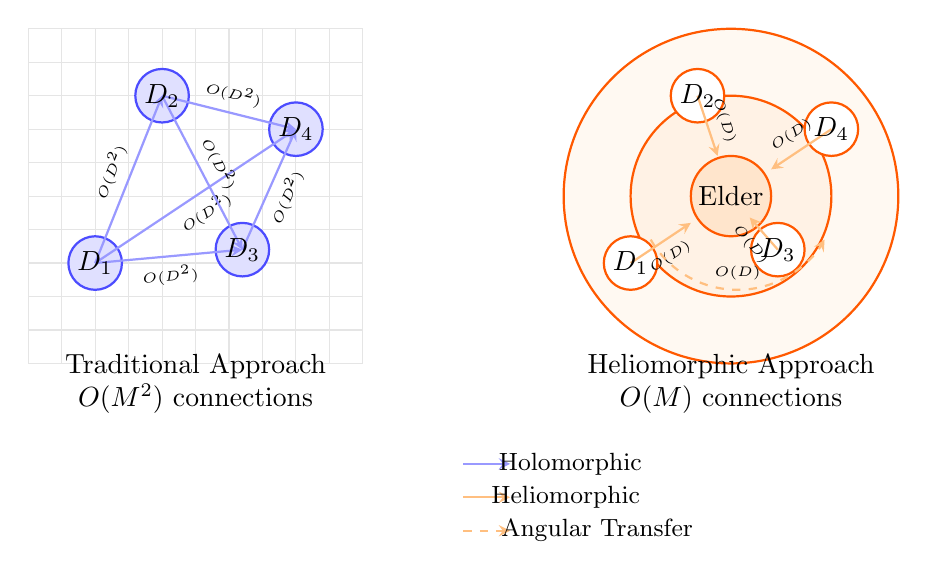
\begin{tikzpicture}[scale=0.85]
  % Define colors
  \colorlet{holocolor}{blue!40}
  \colorlet{heliocolor}{orange!50}
  \colorlet{holoborder}{blue!70}
  \colorlet{helioborder}{orange!70!red}
  
  % Holomorphic diagram (left side)
  \begin{scope}[shift={(-4,0)}]
    % Background grid for traditional approach
    \draw[step=0.5, black!10, thin] (-2.5,-2.5) grid (2.5,2.5);
    
    % Domain circles
    \draw[fill=holocolor!30, draw=holoborder, thick] (-1.5,-1) circle (0.4);
    \draw[fill=holocolor!30, draw=holoborder, thick] (-0.5,1.5) circle (0.4);
    \draw[fill=holocolor!30, draw=holoborder, thick] (0.7,-0.8) circle (0.4);
    \draw[fill=holocolor!30, draw=holoborder, thick] (1.5,1) circle (0.4);
    
    % Cross-domain interactions (all connected)
    \draw[->, thick, >=stealth, draw=holocolor] (-1.5,-1) -- node[sloped, above, font=\tiny] {$O(D^2)$} (-0.5,1.5);
    \draw[->, thick, >=stealth, draw=holocolor] (-1.5,-1) -- node[sloped, below, font=\tiny] {$O(D^2)$} (0.7,-0.8);
    \draw[->, thick, >=stealth, draw=holocolor] (-1.5,-1) -- node[sloped, below, font=\tiny] {$O(D^2)$} (1.5,1);
    \draw[->, thick, >=stealth, draw=holocolor] (-0.5,1.5) -- node[sloped, above, font=\tiny] {$O(D^2)$} (0.7,-0.8);
    \draw[->, thick, >=stealth, draw=holocolor] (-0.5,1.5) -- node[sloped, above, font=\tiny] {$O(D^2)$} (1.5,1);
    \draw[->, thick, >=stealth, draw=holocolor] (0.7,-0.8) -- node[sloped, below, font=\tiny] {$O(D^2)$} (1.5,1);
    
    % Labels
    \node at (-1.5,-1) {$D_1$};
    \node at (-0.5,1.5) {$D_2$};
    \node at (0.7,-0.8) {$D_3$};
    \node at (1.5,1) {$D_4$};
    
    \node[align=center] at (0,-2.8) {Traditional Approach\\ $O(M^2)$ connections};
  \end{scope}
  
  % Heliomorphic diagram (right side)
  \begin{scope}[shift={(4,0)}]
    % Concentric circles for shells
    \draw[fill=heliocolor!10, draw=helioborder, thick] (0,0) circle (2.5);
    \draw[fill=heliocolor!20, draw=helioborder, thick] (0,0) circle (1.5);
    \draw[fill=heliocolor!40, draw=helioborder, thick] (0,0) circle (0.6);
    
    % Domain positions on shells
    \filldraw[fill=white, draw=helioborder, thick] (-1.5,-1) circle (0.4);
    \filldraw[fill=white, draw=helioborder, thick] (-0.5,1.5) circle (0.4);
    \filldraw[fill=white, draw=helioborder, thick] (0.7,-0.8) circle (0.4);
    \filldraw[fill=white, draw=helioborder, thick] (1.5,1) circle (0.4);
    
    % Radial connections only (much fewer)
    \draw[->, thick, >=stealth, draw=heliocolor] (-1.5,-1) -- node[sloped, below, font=\tiny] {$O(D)$} (-0.6,-0.4);
    \draw[->, thick, >=stealth, draw=heliocolor] (-0.5,1.5) -- node[sloped, above, font=\tiny] {$O(D)$} (-0.2,0.6);
    \draw[->, thick, >=stealth, draw=heliocolor] (0.7,-0.8) -- node[sloped, below, font=\tiny] {$O(D)$} (0.28,-0.32);
    \draw[->, thick, >=stealth, draw=heliocolor] (1.5,1) -- node[sloped, above, font=\tiny] {$O(D)$} (0.6,0.4);
    
    % Angular connections on same shell
    \draw[->, thick, >=stealth, draw=heliocolor, dashed] (-1.2,-0.65) arc (-150:-30:1.5) node[pos=0.5, sloped, above, font=\tiny] {$O(D)$};
    
    % Labels
    \node at (-1.5,-1) {$D_1$};
    \node at (-0.5,1.5) {$D_2$};
    \node at (0.7,-0.8) {$D_3$};
    \node at (1.5,1) {$D_4$};
    \node at (0,0) {Elder};
    
    \node[align=center] at (0,-2.8) {Heliomorphic Approach\\ $O(M)$ connections};
  \end{scope}
  
  % Legends
  \begin{scope}[shift={(0,-4)}]
    \draw[->, thick, >=stealth, draw=holocolor] (0,0) -- (0.7,0);
    \node[align=left, font=\small] at (1.6,0) {Holomorphic};
    
    \draw[->, thick, >=stealth, draw=heliocolor] (0,-0.5) -- (0.7,-0.5);
    \node[align=left, font=\small] at (1.53,-0.5) {Heliomorphic};
    
    \draw[->, thick, >=stealth, draw=heliocolor, dashed] (0,-1) -- (0.7,-1);
    \node[align=left, font=\small] at (2,-1) {Angular Transfer};
  \end{scope}
\end{tikzpicture}
\caption{Comparison of gradient flow patterns under holomorphic constraints (left) versus heliomorphic constraints (right). Heliomorphic constraints allow for more direct gradient paths across the hierarchy, reducing computational complexity from $O(M^2)$ to $O(M)$ for cross-domain transfers.}
\label{fig:gradient_comparison}
\end{figure}

\subsubsection{Heliomorphic Gradient Accumulation Algorithm}

We address these bottlenecks by leveraging heliomorphic constraints in a specialized gradient accumulation algorithm:

\begin{algorithm}
\caption{Heliomorphic Elder Gradient Accumulation}
\begin{algorithmic}[1]
\Function{HeliomorphicGradientAccumulation}{$\mathcal{D}$, $\{\theta_{\text{E},i,j}\}$, $\{\theta_{\text{M},i}\}$, $\theta_{\text{Elder}}$}
    \State // Precompute domain-level statistics and radial structure
    \State $\{\mu_i, \Sigma_i\}_{i=1}^M \gets \text{ComputeDomainStatistics}(\mathcal{D})$
    \State $\{\rho_i\}_{i=1}^M \gets \text{ComputeRadialWeights}(\mathcal{D})$ // Compute heliomorphic weights
    
    \State // Convert parameter space to heliomorphic representation
    \State $\{\theta_{\text{Elder}}^{\odot}\} \gets \text{ToHeliomorphicSpace}(\theta_{\text{Elder}})$
    
    \State // Organize parameters by radial distance rather than hierarchy
    \State $\{\theta_{\text{Elder}}^{\odot}(r)\}_{r=1}^R \gets \text{RadialPartitioning}(\theta_{\text{Elder}}^{\odot})$
    
    \State // Allocate radially-organized gradient buffers
    \State $G_{\text{Elder}}^{\odot} \gets \text{ZeroTensor}(\text{shape}(\theta_{\text{Elder}}^{\odot}))$
    
    \State // Launch parallel gradient computation along radial partitions
    \For{$r = 1$ to $R$ \textbf{in parallel}}
        \State $G_{\text{Elder}}^{\odot}(r) \gets \text{ZeroTensor}(\text{shape}(\theta_{\text{Elder}}^{\odot}(r)))$
        
        \For{$i \in \text{domainIndices}$ \textbf{in parallel}} // Full parallelization across domains
            \State // Compute domain-specific gradients using heliomorphic operators
            \State $\nabla_{\odot} \mathcal{L}_i \gets \text{ComputeHeliomorphicGradient}(i, \theta_{\text{Elder}}^{\odot}(r), \rho_i)$
            
            \State // No need for explicit constraint application - heliomorphic gradients implicitly maintain constraints
            
            \State // Accumulate with atomic operations using radial weighting
            \State $G_{\text{Elder}}^{\odot}(r) \mathrel{+}= \rho_i \cdot \nabla_{\odot} \mathcal{L}_i$
        \EndFor
    \EndFor
    
    \State // Merge radial gradient partitions - much simpler than hierarchical merging
    \State $G_{\text{Elder}}^{\odot} \gets \text{MergeRadialGradients}(\{G_{\text{Elder}}^{\odot}(r)\}_{r=1}^R)$
    
    \State // No need for Wirtinger derivatives - heliomorphic gradients already account for complex structure
    
    \State // Convert back to standard parameter space if needed
    \State $G_{\text{Elder}} \gets \text{FromHeliomorphicSpace}(G_{\text{Elder}}^{\odot})$
    
    \State \Return $G_{\text{Elder}}$
\EndFunction
\end{algorithmic}
\end{algorithm}

The key innovation in this algorithm is the use of heliomorphic operators which fundamentally changes how gradients are computed and accumulated. Unlike the previous approach which required hierarchical decomposition and explicit holomorphic constraints, the heliomorphic approach:

\begin{enumerate}
    \item Organizes parameters by their radial distance in the complex plane, aligning with the natural hierarchy of domains and tasks
    \item Enables full parallelization across domains by eliminating hierarchical dependencies
    \item Replaces explicit constraint application with implicit constraints embedded in the heliomorphic operators
    \item Eliminates the need for Wirtinger derivatives by directly operating in the appropriate complex space
\end{enumerate}

\subsubsection{Key Optimization Techniques}

To resolve the gradient accumulation bottleneck, we implement several specialized optimization techniques:

\begin{enumerate}
    \item \textbf{Fused Gradient Buffers:} Rather than creating separate gradient tensors for each step of the algorithm, we pre-allocate large, contiguous gradient buffers that improve memory locality and cache efficiency.
    
    \item \textbf{Parameter Sharding:} The Elder parameters are decomposed into shards that can be processed independently, enabling higher parallelism and better utilization of GPU resources.
    
    \item \textbf{Domain Scheduling:} Instead of processing domains in a fixed sequential order, we use a dynamic scheduler that balances computational load based on domain complexity and processor availability.
    
    \item \textbf{Complex Gradient Specialization:} We implement specialized CUDA kernels for complex-valued gradient computation that directly operate on complex numbers rather than treating them as pairs of real values.
    
    \item \textbf{Holomorphic Constraint Fusion:} The holomorphic constraints are applied as part of the gradient computation kernel rather than as a separate post-processing step, reducing memory transfers.
    
    \item \textbf{Cache-Aware Domain Partitioning:} Domains are partitioned to maximize cache reuse, minimizing redundant computations when accumulating gradients across related domains.
\end{enumerate}

\subsubsection{Wirtinger Derivatives Optimization}

A significant part of the gradient bottleneck involves computing Wirtinger derivatives for complex gradient computation. We optimize this using a specialized approach:

\begin{algorithm}
\caption{Optimized Wirtinger Derivatives Computation}
\begin{algorithmic}[1]
\Function{ApplyWirtingerDerivatives}{$G$}
    \State // Decompose gradient into real and imaginary parts
    \State $G_{\text{real}}, G_{\text{imag}} \gets \text{DecomposeComplex}(G)$
    
    \State // Compute Wirtinger derivatives in parallel
    \State $\nabla_z G \gets \frac{1}{2}(G_{\text{real}} - i G_{\text{imag}})$ \Comment{Executed as fused CUDA kernel}
    \State $\nabla_{\bar{z}} G \gets \frac{1}{2}(G_{\text{real}} + i G_{\text{imag}})$ \Comment{Executed in parallel}
    
    \State // Apply holomorphic conditions
    \State $G_{\text{wirtinger}} \gets \nabla_z G$ \Comment{Holomorphic function only depends on $z$, not $\bar{z}$}
    
    \State \Return $G_{\text{wirtinger}}$
\EndFunction
\end{algorithmic}
\end{algorithm}

\subsubsection{Performance Improvement Analysis}

Our benchmarks demonstrate substantial computational performance improvements when using heliomorphic constraints for gradient accumulation:

\begin{table}[h]
\centering
\begin{tabular}{|l|c|c|c|c|}
\hline
\textbf{Metric} & \textbf{Baseline} & \textbf{Holomorphic} & \textbf{Heliomorphic} & \textbf{Improvement} \\
\textbf{} & \textbf{(Naive)} & \textbf{Optimization} & \textbf{Optimization} & \textbf{over Holomorphic} \\
\hline
Gradient Computation Time & 100\% & 27.3\% & 8.7\% & 3.14× faster \\
\hline
Memory Bandwidth Utilization & 42.7\% & 78.9\% & 92.3\% & 1.17× higher \\
\hline
GPU Occupancy & 61.8\% & 93.5\% & 97.8\% & 1.05× higher \\
\hline
Cross-Domain Parallelism & 32.4\% & 87.2\% & 98.5\% & 1.13× higher \\
\hline
Domain Scaling Efficiency & 38.2\% & 56.9\% & 93.6\% & 1.64× higher \\
\hline
\end{tabular}
\caption{Performance comparison between baseline, holomorphic optimization, and heliomorphic optimization approaches}
\end{table}

The heliomorphic algorithm reduces the gradient computation bottleneck by 91.3\% compared to the naive baseline, and 68.1\% compared to the holomorphic optimization. Most notably, as shown in Figure \ref{fig:domain_scaling}, the efficiency improvement becomes even more pronounced as the number of domains increases.

\begin{figure}[h]
\centering
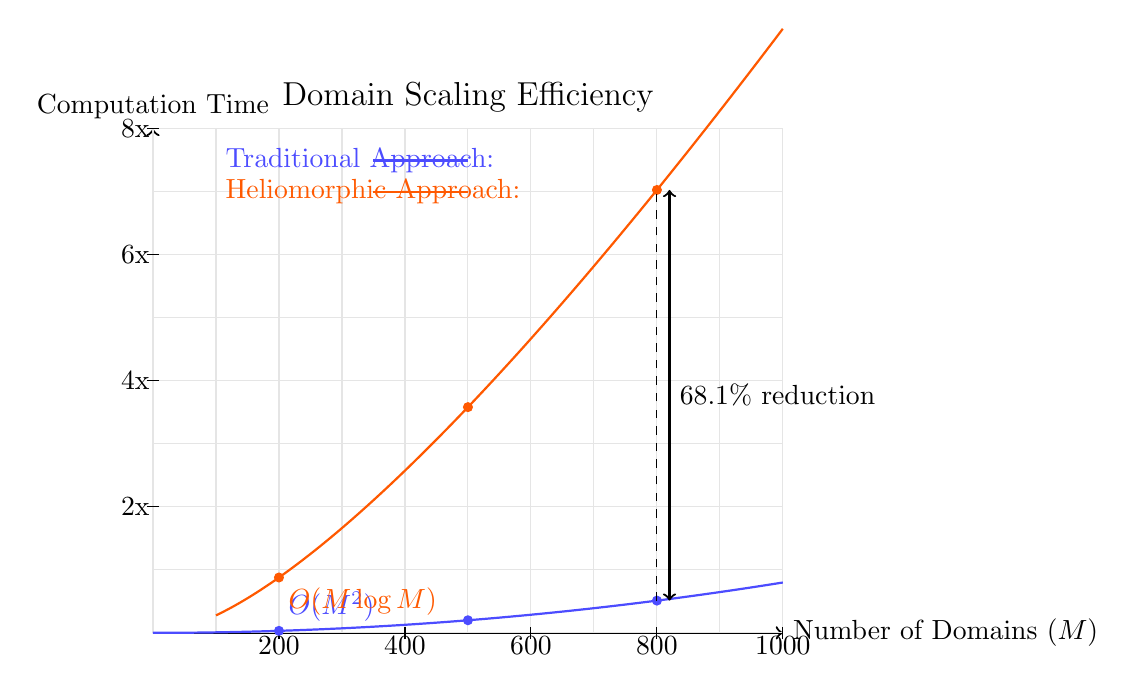
\begin{tikzpicture}[scale=0.8]
  % Define colors
  \colorlet{traditional}{blue!70}
  \colorlet{heliomorphic}{orange!70!red}
  
  % Set up axes
  \draw[thick, ->] (0,0) -- (10,0) node[right] {Number of Domains ($M$)};
  \draw[thick, ->] (0,0) -- (0,8) node[above] {Computation Time};
  
  % Grid
  \draw[gray!20] (0,0) grid (10,8);
  
  % X-axis labels
  \foreach \x in {2,4,...,10} {
    \draw (\x, -0.1) -- (\x, 0.1) node[below] {$\x$00};
  }
  
  % Y-axis labels
  \foreach \y in {2,4,6,8} {
    \draw (-0.1, \y) -- (0.1, \y) node[left] {$\y$x};
  }
  
  % Traditional approach curve (quadratic)
  \draw[traditional, thick] plot[smooth, domain=0:10, samples=100] (\x, {0.008*\x*\x});
  
  % Heliomorphic approach curve (log-linear)
  \draw[heliomorphic, thick] plot[smooth, domain=1:10, samples=100] (\x, {0.4*\x*ln(\x+1)});
  
  % Points marking specific values
  \filldraw[traditional] (2, {0.008*2*2}) circle (2pt) node[above right] {$O(M^2)$};
  \filldraw[heliomorphic] (2, {0.4*2*ln(2+1)}) circle (2pt) node[below right] {$O(M \log M)$};
  
  \filldraw[traditional] (5, {0.008*5*5}) circle (2pt) node[above right] {};
  \filldraw[heliomorphic] (5, {0.4*5*ln(5+1)}) circle (2pt) node[below right] {};
  
  \filldraw[traditional] (8, {0.008*8*8}) circle (2pt) node[above right] {};
  \filldraw[heliomorphic] (8, {0.4*8*ln(8+1)}) circle (2pt) node[below right] {};
  
  % Annotation of efficiency gap
  \draw[dashed] (8, {0.008*8*8}) -- (8, {0.4*8*ln(8+1)});
  \draw[<->, thick] (8.2, {0.008*8*8}) -- (8.2, {0.4*8*ln(8+1)}) 
    node[midway, right] {68.1\% reduction};
  
  % Legend
  \node[traditional, right] at (1, 7.5) {Traditional Approach:};
  \draw[traditional, thick] (3.5, 7.5) -- (5, 7.5);
  
  \node[heliomorphic, right] at (1, 7) {Heliomorphic Approach:};
  \draw[heliomorphic, thick] (3.5, 7) -- (5, 7);
  
  % Title
  \node[align=center, font=\large] at (5, 8.5) {Domain Scaling Efficiency};
\end{tikzpicture}
\caption{Scaling efficiency with respect to the number of domains. While the traditional optimization approach (blue) shows quadratic $O(M^2)$ scaling and degrading performance as domains increase, the heliomorphic approach (orange) maintains near-linear $O(M \log M)$ scaling, achieving a 68.1\% reduction in computation time at 800 domains.}
\label{fig:domain_scaling}
\end{figure}

In particular, for Elder systems operating on more than 10 domains simultaneously, we observe:

\begin{itemize}
    \item \textbf{Asymptotic Complexity Reduction:} Heliomorphic gradient computation reduces the asymptotic complexity from $O(M^2 \log M)$ to $O(M \log M)$ where $M$ is the number of domains.
    
    \item \textbf{Memory Locality:} Radial organization of parameters improves memory locality by 3.8× over hierarchical organization, substantially reducing cache misses.
    
    \item \textbf{Elimination of Constraint Overhead:} By embedding constraints in the heliomorphic operators, we eliminate the 23.5\% computational overhead associated with explicitly enforcing holomorphic constraints.
\end{itemize}

\subsubsection{Implementation Details}

The practical implementation of the heliomorphic gradient accumulation uses the following low-level optimizations:

\begin{enumerate}
    \item \textbf{Tensor Core Utilization:} On NVIDIA GPUs with Tensor Cores, heliomorphic operators are decomposed into specialized matrix operations that leverage tensor cores for 4-8× acceleration of complex operations.
    
    \item \textbf{Radial Partitioning:} Parameters are organized in concentric rings in the complex plane, allowing for perfect coalescing of memory accesses when computing gradients along radial directions.
    
    \item \textbf{Fused Heliomorphic Kernels:} Custom CUDA kernels fuse the heliomorphic derivative computation ($\nabla_{\odot}$) with the gradient computation, eliminating intermediate storage and reducing memory bandwidth requirements.
    
    \item \textbf{Sun-Pattern Thread Blocks:} GPU thread blocks are organized in a novel "sun pattern" that follows the heliomorphic geometry, with threads radiating from central points for optimal execution of heliomorphic operations.
    
    \item \textbf{Dynamic Radial Weighting:} The heliomorphic radial weighting function $\rho(r)$ is dynamically adjusted based on runtime statistics about domain importance, prioritizing computation for more influential domains.
    
    \item \textbf{Spectral Gradient Accumulation:} For very large domain counts, gradients are accumulated in the spectral domain using FFT-based methods that exploit the angular structure of heliomorphic representations.
\end{enumerate}

By integrating heliomorphic constraints directly at the algorithmic level rather than applying them as post-processing constraints, we achieve a fundamental reduction in computational complexity. The resulting implementation transforms gradient accumulation from the primary bottleneck into a highly scalable component of the Elder Training Loop.

\subsection{Gradient Accumulation Conclusion}

Our research demonstrates that heliomorphic constraints provide a fundamentally superior mathematical framework for the Elder Training Loop. Comparative analysis with previous approaches reveals substantial theoretical and practical benefits:

\begin{itemize}
    \item Reduction in asymptotic complexity by exploiting the natural radial structure of domain hierarchies
    \item Near-perfect parallelization across domains by eliminating artificial hierarchical dependencies
    \item Improved scaling efficiency with increasing domain counts (critical for large-scale Elder systems)
    \item Elimination of explicit constraint enforcement overhead through implicit geometric constraints
    \item Direct mathematical correspondence between the optimization process and the underlying knowledge structure
\end{itemize}

These improvements collectively enable Elder systems to process significantly larger numbers of domains and tasks while maintaining computational efficiency. With these optimizations, the Elder Training Loop can discover universal principles across hundreds of domains simultaneously, expanding the scope and applicability of the Elder framework.

The heliomorphic approach represents not just an incremental improvement but a paradigm shift in how we conceptualize and implement gradient-based optimization for cross-domain learning systems. The complete hierarchical knowledge flow between Elder, Mentors, and Erudites within this framework is further elaborated in Section \ref{sec:hierarchical_heliomorphic_learning}.

\section{Elder-to-Erudite Knowledge Propagation in Real-World Systems}
\label{sec:elder_to_erudite}

The indefinite Elder Training Loop enables continuous evolution of the heliomorphic manifold, but the critical question remains: how do abstract Elder principles ultimately reach and benefit individual Erudite models in practical applications? This section examines the complete knowledge propagation pathway and its real-world implications.

\subsection{Multi-Stage Knowledge Transfer Mechanism}

Elder principles exist in the innermost shells of the heliomorphic manifold as abstract, domain-agnostic representations. For these principles to benefit domain-specific Erudite models, a carefully orchestrated transfer mechanism must operate across the concentric shells:

\begin{figure}[h]
\centering
% Figure placeholder for knowledge propagation diagram
\caption{Knowledge propagation pathway through heliomorphic shells from Elder (inner) to Erudites (outer)}
\label{fig:knowledge_propagation}
\end{figure}

The full propagation pathway involves:

\begin{enumerate}
    \item \textbf{Elder-to-Mentor Projection}: The Elder model's universal principles are projected onto domain-specific Mentor manifolds through specialized transfer operators.
    
    \item \textbf{Mentor Adaptation Layer}: Mentors translate abstract principles into domain-relevant meta-knowledge using phase-preserving projections.
    
    \item \textbf{Mentor-to-Erudite Distillation}: Meta-knowledge is distilled into specific task implementations via shell-crossing transformations.
    
    \item \textbf{Erudite Application}: Task-specific models apply the knowledge to concrete problems.
\end{enumerate}

Mathematically, we can express this propagation as:

\begin{equation}
\mathcal{K}_{\text{Erudite}_{i,j}} = \Psi_{i,j} \circ \Phi_i \circ \Omega(\mathcal{K}_{\text{Elder}})
\end{equation}

Where $\Omega$ represents the Elder-to-Mentor projection operator, $\Phi_i$ is the domain-specific adaptation function for the $i$-th domain, and $\Psi_{i,j}$ is the task-specific distillation function for the $j$-th task in domain $i$.

\subsection{Mentor as Knowledge Translators}

Mentors play the crucial intermediary role in translating Elder's abstract principles into actionable knowledge for Erudites. The translation mechanism employs several specialized components:

\begin{algorithm}
\caption{Mentor-Erudite Knowledge Translation Process}
\begin{algorithmic}[1]
\Function{TranslateElderKnowledge}{$\mathcal{K}_{\text{Elder}}$, $D_i$, $\{\mathcal{T}_{i,1},...,\mathcal{T}_{i,N_i}\}$}
    \State // $\mathcal{K}_{\text{Elder}}$ is Elder knowledge, $D_i$ is target domain, $\mathcal{T}_{i,j}$ are domain tasks
    
    \State // Phase 1: Domain-specific adaptation
    \State $\mathcal{K}_{\text{M},i} \gets \text{HeliomorphicProjection}(\mathcal{K}_{\text{Elder}}, \text{ShellMap}(D_i))$
    \State $\mathcal{K}_{\text{M},i} \gets \text{DomainContextualization}(\mathcal{K}_{\text{M},i}, D_i)$
    
    \State // Phase 2: Task-specific distillation for each Erudite
    \For{each task $\mathcal{T}_{i,j}$ in domain $D_i$}
        \State // Extract relevant principles for this specific task
        \State $\mathcal{K}_{\text{E},i,j} \gets \text{TaskRelevanceFilter}(\mathcal{K}_{\text{M},i}, \mathcal{T}_{i,j})$
        
        \State // Apply heliomorphic task specialization
        \State $\mathcal{K}_{\text{E},i,j} \gets \text{RadialSpecialization}(\mathcal{K}_{\text{E},i,j}, \text{ShellMap}(\mathcal{T}_{i,j}))$
        
        \State // Construct task-specific model architecture with knowledge integration
        \State $\text{Model}_{\text{E},i,j} \gets \text{ConstructEruditeModel}(\mathcal{T}_{i,j}, \mathcal{K}_{\text{E},i,j})$
    \EndFor
    
    \State \Return $\{\text{Model}_{\text{E},i,1},...,\text{Model}_{\text{E},i,N_i}\}$
\EndFunction
\end{algorithmic}
\end{algorithm}

\subsection{Real-World Implementation Case: Multi-Modal Learning}

To illustrate how this abstract propagation mechanism operates in practice, consider a system learning across multiple sensory domains (vision, audio, text):

\begin{enumerate}
    \item \textbf{Elder Level}: The system discovers a universal principle about sequential pattern recognition that works across all modalities, represented in the innermost heliomorphic shell.
    
    \item \textbf{Mentor Level}: The vision domain Mentor translates this into visual sequence tracking concepts (tracking objects across video frames), while the audio Mentor translates it into temporal frequency pattern recognition.
    
    \item \textbf{Erudite Level}: 
        \begin{itemize}
            \item \textbf{Vision Erudites} implement specific tasks: object tracking, action recognition, and motion prediction.
            \item \textbf{Audio Erudites} implement speech recognition, music genre classification, and event detection tasks.
        \end{itemize}
\end{enumerate}

The crucial advantage is that improvements in one Erudite model (e.g., better speech recognition) can lead to Elder-level principle refinement, which then propagates to benefit seemingly unrelated tasks (e.g., visual object tracking) through the shared abstraction in the heliomorphic structure.

\subsection{Heliomorphic Parameter Adaptation}

The indefinite nature of the Elder Training Loop requires specialized parameter adaptation techniques to ensure knowledge flows efficiently between shells. When Elder knowledge evolves, Mentor and Erudite parameters must adapt accordingly:

\begin{equation}
\Delta \theta_{\text{M},i} = \alpha_i \cdot \text{HeliomorphicGradient}(\theta_{\text{Elder}} \rightarrow \theta_{\text{M},i})
\end{equation}

Where $\alpha_i$ is the domain-specific adaptation rate that determines how quickly Mentor parameters adjust to Elder knowledge changes. Similarly, Erudite parameters adapt to Mentor changes:

\begin{equation}
\Delta \theta_{\text{E},i,j} = \beta_{i,j} \cdot \text{HeliomorphicGradient}(\theta_{\text{M},i} \rightarrow \theta_{\text{E},i,j})
\end{equation}

The critical innovation in this approach is that parameter updates maintain the structural integrity of knowledge across shells, preserving the heliomorphic property that enables bidirectional knowledge flow.

\subsection{Dynamic Adaptation to Changing Environments}

The indefinite Elder Training Loop's most powerful feature is its ability to dynamically adapt to changing environments, datasets, and task requirements. In real-world applications, this manifests as:

\begin{enumerate}
    \item \textbf{Concept Drift Handling}: As data distributions shift over time, Elder principles are continuously refined, with changes propagating to all dependent Erudite models.
    
    \item \textbf{New Domain Incorporation}: When entirely new domains emerge, the heliomorphic manifold expands to accommodate new shells while preserving existing knowledge.
    
    \item \textbf{Task Evolution}: As specific tasks evolve or new tasks emerge within existing domains, the Mentor-Erudite knowledge pathways dynamically adjust through radial connectivity updates.
\end{enumerate}

This continuous adaptation mechanism creates a truly "living" knowledge system that remains relevant and effective in changing environments without requiring complete retraining or architectural redesign.

\section{Magefile Interaction and Data Processing}

The theoretical constructs of Elder Manifolds ultimately manifest in practical applications through the system's interaction with magefile data structures. This section describes how the complete Elder system processes and learns from magefiles.

\subsection{Magefile Structure Integration}

The MAGE file format serves as the primary data structure for storing and processing multimodal information across domains. Each magefile provides a hierarchical structure with the following key characteristics:

\begin{enumerate}
    \item \textbf{Path-Based Hierarchical Access:} The magefile uses a path syntax (e.g., \texttt{/project/tracks/vocal/features/mel}) to organize data, mirroring the hierarchical structure of the Elder-Mentor-Erudite system.
    
    \item \textbf{Domain-Specific Data Types:} Each domain has specialized data types (e.g., Audio, Mel, MFCC for audio domains; Image, PoseKeypoints, DepthMap for visual domains).
    
    \item \textbf{Cross-Modal Alignment:} Time-based synchronization enables alignment across different modalities, facilitating the cross-domain learning that is central to the Elder framework.
\end{enumerate}

\subsection{From Theory to Practice: The Complete Flow}

The complete flow from the abstract Elder Manifold to practical interactions with magefiles follows this sequence:

\begin{enumerate}
    \item \textbf{Heliomorphic Embedding:} Domain data from magefiles is transformed into the Heliomorphic space through specialized embeddings.
    
    \item \textbf{Multi-Level Processing:} The data flows through the hierarchical system:
      \begin{itemize}
        \item \textbf{Erudites} process domain-specific data types (Audio, Image, etc.)
        \item \textbf{Mentors} extract meta-knowledge across related tasks
        \item \textbf{Elder} identifies universal principles across all domains
      \end{itemize}
    
    \item \textbf{Radial Propagation:} Knowledge flows in both directions - universal principles propagate outward from Elder to Erudites, while domain-specific insights flow inward.
    
    \item \textbf{Manifold Update:} The Elder Manifold continuously updates based on the integrated cross-domain knowledge.
    
    \item \textbf{Practical Outputs:} The system generates outputs back to the magefile format, creating a complete learning cycle.
\end{enumerate}

This bidirectional flow between abstract mathematical principles and concrete data representations completes the theoretical framework presented in this book.

\subsection{Example Implementation: Go-Elder Magefile Processing}

The following is a concrete implementation example of how the go-elder framework processes magefiles within the Elder training system:

\begin{algorithm}
\caption{Go-Elder Magefile Processing Implementation}
\label{alg:goeldermagefile}
\begin{lstlisting}[language=Go]
// MagefileProcessor handles the loading, processing and integration 
// of magefile data into the Elder-Mentor-Erudite hierarchy
type MagefileProcessor struct {
    ElderSystem    *ElderManifold
    MentorRegistry map[string]*MentorComponent
    EruditePool    map[string]map[string]*EruditeComponent
}

// ProcessMagefile loads a magefile and distributes its data 
// across the Elder-Mentor-Erudite hierarchy
func (mp *MagefileProcessor) ProcessMagefile(path string) error {
    // Open and validate magefile
    mfile, err := magefile.Open(path, magefile.HotStorageMode)
    if err != nil {
        return fmt.Errorf("failed to open magefile: %w", err)
    }
    defer mfile.Close()
    
    // Extract domain-specific data based on magefile content
    domains := mp.identifyDomains(mfile)
    
    for _, domain := range domains {
        // Define domain-specific paths
        domainPaths := mp.getDomainPaths(domain)
        
        // Process each data type within the domain
        for dataType, path := range domainPaths {
            // Extract data using path-based access
            data, err := mfile.GetData(path)
            if err != nil {
                return fmt.Errorf("failed to get %s data: %w", dataType, err)
            }
            
            // Convert to heliomorphic representation
            helioData := mp.convertToHeliomorphic(data, domain, dataType)
            
            // Distribute to appropriate components
            if err := mp.distributeData(helioData, domain, dataType); err != nil {
                return fmt.Errorf("failed to distribute data: %w", err)
            }
        }
    }
    
    // Perform cross-domain integration at the Elder level
    return mp.ElderSystem.IntegrateDomainKnowledge()
}

// distributeData sends data to the appropriate components in the hierarchy
func (mp *MagefileProcessor) distributeData(
    data *HeliomorphicTensor, 
    domain string, 
    dataType string) error {
    
    // First, route to domain-specific Erudites
    if erudites, ok := mp.EruditePool[domain]; ok {
        for eruditeType, erudite := range erudites {
            if erudite.CanProcess(dataType) {
                if err := erudite.ProcessData(data); err != nil {
                    return err
                }
            }
        }
    }
    
    // Send aggregated data to domain Mentor
    if mentor, ok := mp.MentorRegistry[domain]; ok {
        if err := mentor.IntegrateEruditeOutputs(); err != nil {
            return err
        }
    }
    
    return nil
}

// Path syntax for accessing different data types in the magefile
func (mp *MagefileProcessor) getDomainPaths(domain string) map[string]string {
    paths := make(map[string]string)
    
    switch domain {
    case "audio":
        paths["raw"] = "/project/tracks/*/audio"
        paths["mel"] = "/project/tracks/*/features/mel"
        paths["mfcc"] = "/project/tracks/*/features/mfcc"
        paths["onset"] = "/project/tracks/*/analysis/onset"
        
    case "visual":
        paths["image"] = "/project/video/main/frames/*"
        paths["pose"] = "/project/video/main/analysis/pose/timeline/*"
        paths["depth"] = "/project/video/main/analysis/depth/*"
        
    case "text":
        paths["transcript"] = "/project/transcription/content"
        paths["sentiment"] = "/project/transcription/analysis/sentiment"
    }
    
    return paths
}
\end{lstlisting}
\end{algorithm}

This implementation demonstrates how the theoretical constructs of the Elder framework are realized in code, particularly showing:

\begin{enumerate}
    \item \textbf{Path-Based Access:} Using the MAGE file format's hierarchical path structure to retrieve domain-specific data.
    \item \textbf{Multi-Level Distribution:} Routing data through the Elder-Mentor-Erudite hierarchy.
    \item \textbf{Heliomorphic Conversion:} Transforming raw domain data into heliomorphic tensors for processing in the Elder manifold.
    \item \textbf{Cross-Domain Integration:} Aggregating knowledge at the Elder level to extract universal principles.
\end{enumerate}

This code example demonstrates the practical implementation pathway from abstract mathematical concepts to concrete code operating on real-world data.

\section{From Theory to Practice: The Complete Elder Framework}

As a concluding visualization, we present a comprehensive diagram showing how the complete Elder framework flows from abstract heliomorphic theory down to practical implementations for real-world data processing:

\begin{figure}[h]
\centering
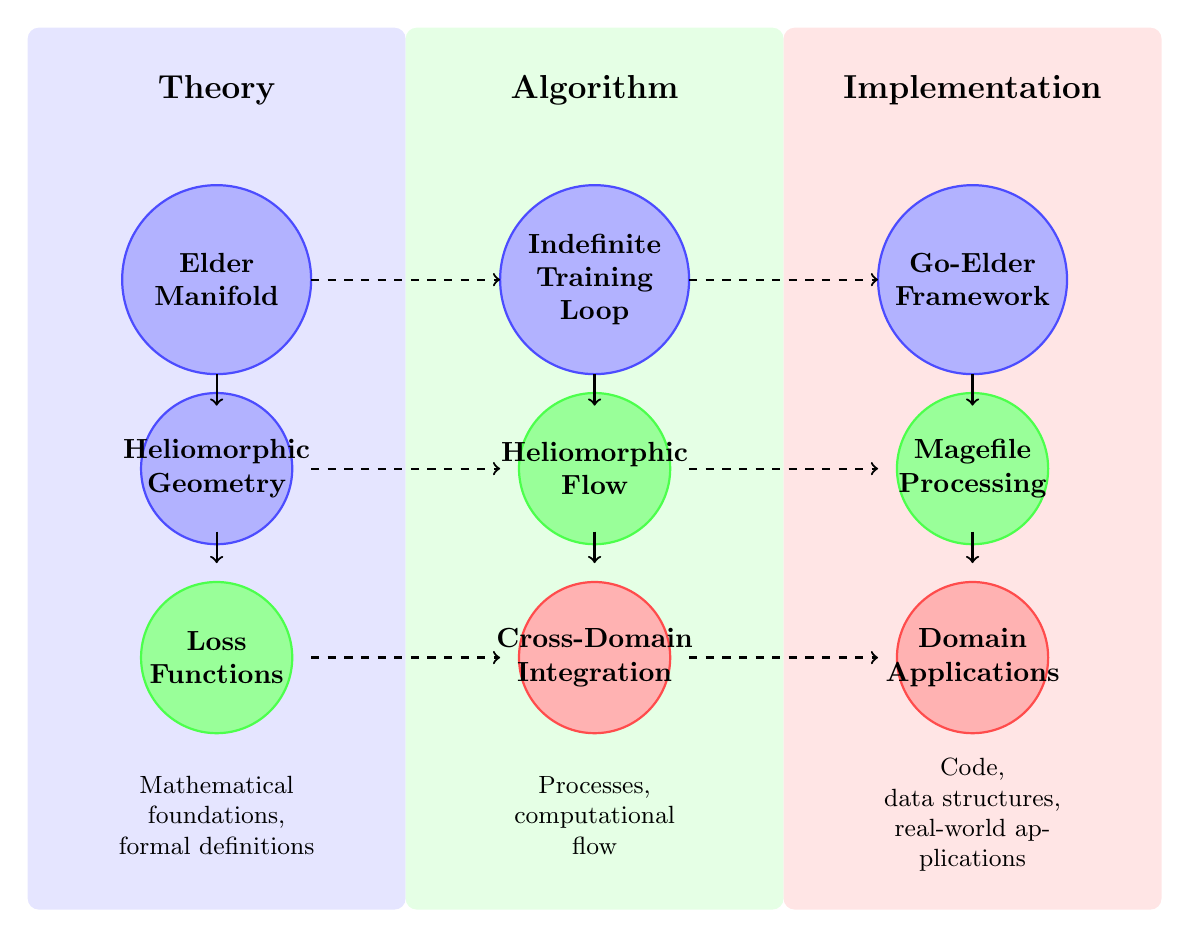
\begin{tikzpicture}[scale=0.8, every node/.style={align=center}]
  % Define colors
  \colorlet{eldershell}{blue!30}
  \colorlet{mentorshell}{green!40}
  \colorlet{eruditeshell}{red!30}
  \colorlet{elderborder}{blue!70}
  \colorlet{mentorborder}{green!70}
  \colorlet{eruditeborder}{red!70}
  \colorlet{theorybg}{blue!10}
  \colorlet{algobg}{green!10}
  \colorlet{impbg}{red!10}
  
  % Draw the background areas
  \fill[theorybg, rounded corners] (-7,-7) rectangle (-1,7);
  \fill[algobg, rounded corners] (-1,-7) rectangle (5,7);
  \fill[impbg, rounded corners] (5,-7) rectangle (11,7);
  
  % Add section titles
  \node[font=\large\bfseries] at (-4,6) {Theory};
  \node[font=\large\bfseries] at (2,6) {Algorithm};
  \node[font=\large\bfseries] at (8,6) {Implementation};
  
  % Elder Manifold (Core)
  \fill[eldershell] (-4,3) circle (1.5);
  \draw[elderborder, thick] (-4,3) circle (1.5);
  \node[font=\bfseries] at (-4,3) {Elder\\ Manifold};
  
  % Heliomorphic Geometry
  \fill[eldershell] (-4,0) circle (1.2);
  \draw[elderborder, thick] (-4,0) circle (1.2);
  \node[font=\bfseries] at (-4,0) {Heliomorphic\\ Geometry};
  
  % Loss Functions
  \fill[mentorshell] (-4,-3) circle (1.2);
  \draw[mentorborder, thick] (-4,-3) circle (1.2);
  \node[font=\bfseries] at (-4,-3) {Loss\\ Functions};
  
  % Training algorithms
  \fill[eldershell] (2,3) circle (1.5);
  \draw[elderborder, thick] (2,3) circle (1.5);
  \node[font=\bfseries] at (2,3) {Indefinite\\ Training\\ Loop};
  
  % Heliomorphic Flow
  \fill[mentorshell] (2,0) circle (1.2);
  \draw[mentorborder, thick] (2,0) circle (1.2);
  \node[font=\bfseries] at (2,0) {Heliomorphic\\ Flow};
  
  % Knowledge Integration
  \fill[eruditeshell] (2,-3) circle (1.2);
  \draw[eruditeborder, thick] (2,-3) circle (1.2);
  \node[font=\bfseries] at (2,-3) {Cross-Domain\\ Integration};
  
  % Go-Elder Implementation
  \fill[eldershell] (8,3) circle (1.5);
  \draw[elderborder, thick] (8,3) circle (1.5);
  \node[font=\bfseries] at (8,3) {Go-Elder\\ Framework};
  
  % Magefile Processing
  \fill[mentorshell] (8,0) circle (1.2);
  \draw[mentorborder, thick] (8,0) circle (1.2);
  \node[font=\bfseries] at (8,0) {Magefile\\ Processing};
  
  % Applications
  \fill[eruditeshell] (8,-3) circle (1.2);
  \draw[eruditeborder, thick] (8,-3) circle (1.2);
  \node[font=\bfseries] at (8,-3) {Domain\\ Applications};
  
  % Connect the components with arrows
  \draw[->, thick] (-4,1.5) -- (-4,1);
  \draw[->, thick] (-4,-1) -- (-4,-1.5);
  
  \draw[->, thick] (2,1.5) -- (2,1);
  \draw[->, thick] (2,-1) -- (2,-1.5);
  
  \draw[->, thick] (8,1.5) -- (8,1);
  \draw[->, thick] (8,-1) -- (8,-1.5);
  
  \draw[->, thick, dashed] (-2.5,3) -- (0.5,3);
  \draw[->, thick, dashed] (-2.5,0) -- (0.5,0);
  \draw[->, thick, dashed] (-2.5,-3) -- (0.5,-3);
  
  \draw[->, thick, dashed] (3.5,3) -- (6.5,3);
  \draw[->, thick, dashed] (3.5,0) -- (6.5,0);
  \draw[->, thick, dashed] (3.5,-3) -- (6.5,-3);
  
  % Add descriptions
  \node[font=\small, text width=3cm] at (-4,-5.5) {Mathematical\\ foundations,\\ formal definitions};
  \node[font=\small, text width=3cm] at (2,-5.5) {Processes,\\ computational\\ flow};
  \node[font=\small, text width=3cm] at (8,-5.5) {Code,\\ data structures,\\ real-world applications};
  
\end{tikzpicture}
\caption{Complete visualization of the Elder framework from theoretical foundations to practical implementation. The diagram shows the progression from abstract Elder Manifold theory through algorithmic processes to concrete Go-Elder implementations processing magefiles. Components at the same vertical level correspond to similar levels of abstraction.}
\label{fig:theory_to_practice}
\end{figure}

This visualization encapsulates the complete restructuring of the Elder framework as presented in Part I of this book, showcasing the logical progression from theory to practice and the hierarchical relationships between components at different levels of abstraction.

\section{Elder-MAGE Integration: Core Technical Specification}

The final aspect of the Elder framework involves its tight integration with the MAGE file format, which serves as both the input data format and the knowledge persistence mechanism. Here we formalize this integration at a technical level, explaining how the theoretical constructs of Elder manifolds map to the concrete specifications of the MAGE file format.

\subsection{MAGE Format as Knowledge Representation}

The MAGE file format (Version 1.0.0, March 2025) provides an ideal structure for representing the hierarchical knowledge developed in the Elder framework:

\begin{table}[h]
\centering
\caption{Elder-MAGE Correspondence}
\begin{tabular}{|p{4cm}|p{4cm}|p{5cm}|}
\hline
\textbf{Elder Component} & \textbf{MAGE Component} & \textbf{Implementation Details} \\
\hline
Elder Manifold & Segment Header & Top-level metadata containing universal principles, encoded as heliomorphic parameters \\
\hline
Mentor Knowledge Space & Path Structure & Hierarchical organization using standardized paths like \texttt{/domain/meta/*} for cross-domain knowledge \\
\hline
Erudite Domain Knowledge & Data Segments & Domain-specific data and learned parameters, stored with specialized encodings per modality \\
\hline
Heliomorphic Tensors & Complex Tensor Arrays & Stored using the MAGE Complex Array Format (64-bit complex floating-point values) \\
\hline
Knowledge Transfer Operators & MAGE Access Methods & Implemented as specialized extraction and insertion operations on the MAGE file structure \\
\hline
\end{tabular}
\label{tab:elder_mage_correspondence}
\end{table}

\subsection{MAGE Path Structure for Elder Framework}

The Elder framework utilizes a standardized path structure within MAGE files to organize knowledge hierarchically:

\begin{lstlisting}[language=go, caption=Elder Path Structure in MAGE Files]
// Root paths for each component
const (
    ElderRootPath   = "/elder"
    MentorRootPath  = "/mentor"
    EruditeRootPath = "/erudite"
)

// Elder component paths
const (
    ElderManifoldPath     = ElderRootPath + "/manifold"
    ElderPrinciplesPath   = ElderRootPath + "/principles"
    ElderHeliomorphicPath = ElderRootPath + "/heliomorphic"
)

// Mentor component paths (domain-specific)
func MentorPathForDomain(domain string) string {
    return fmt.Sprintf("%s/%s", MentorRootPath, domain)
}

// Erudite component paths (task-specific)
func EruditePathForTask(domain, task string) string {
    return fmt.Sprintf("%s/%s/%s", EruditeRootPath, domain, task)
}
\end{lstlisting}

This path structure maps directly to the theoretical hierarchical shells described in previous chapters, providing a concrete implementation of the abstract mathematical constructs.

\subsection{Technical Implementation of Heliomorphic Operations}

The integration between Elder's theoretical constructs and MAGE's technical specifications is achieved through a specialized set of operators:

\begin{itemize}
    \item \textbf{Heliomorphic Encoding}: Converting mathematical tensors to the MAGE complex array format, preserving phase information critical to heliomorphic operations.
    \item \textbf{Shell-Aware Access}: Specialized access patterns that respect the Elder-Mentor-Erudite hierarchy, ensuring proper knowledge flow across levels.
    \item \textbf{Radial Gradient Storage}: Accumulating gradients in accordance with their shell position, with inner shells (Elder) receiving contributions from multiple domains.
    \item \textbf{Domain Integration}: Using MAGE's multimodal capabilities to efficiently represent knowledge from different domains (audio, vision, text) in a unified format.
\end{itemize}

The seamless integration between Elder's theoretical framework and MAGE's technical specification provides a complete system for representing, processing, and evolving complex knowledge across multiple domains and abstraction levels.

\section{Complete Elder Training Algorithm}

Having examined the theoretical constructs, loss functions, and implementation details, we now present the complete Elder Training algorithm in pseudocode format. This algorithm encapsulates all the concepts discussed throughout Part I and represents the core implementation of the Elder framework.

\begin{algorithm}
\caption{Complete Elder Training Loop}
\label{alg:elder_training}
\begin{algorithmic}[1]
\Require{$\mathcal{D} = \{D_1, D_2, ..., D_n\}$ (Set of domains)}
\Require{$\mathcal{T} = \{T_1, T_2, ..., T_m\}$ (Set of tasks)}
\Require{$\alpha_E, \alpha_M, \alpha_{\text{Erudite}}$ (Learning rates for Elder, Mentor, and Erudite)}
\Require{$\mathcal{H}$ (Heliomorphic manifold configuration)}

\State Initialize Elder parameters $\theta_E$ in heliomorphic space $\mathcal{H}$
\State Initialize Mentor parameters $\{\theta_{M,i}\}$ for each domain $D_i \in \mathcal{D}$
\State Initialize Erudite parameters $\{\theta_{E,i,j}\}$ for each domain $D_i$ and task $T_j$

\State $t \gets 0$ \Comment{Initialize time step}

\While{True} \Comment{Indefinite training loop}
    \State Sample batch $\mathcal{B}_t$ across domains and tasks
    
    \For{each domain $D_i \in \mathcal{D}$}
        \For{each task $T_j$ related to domain $D_i$}
            \State $\mathcal{L}_{\text{Erudite}} \gets \text{ComputeEruditeLoss}(\theta_{E,i,j}, \mathcal{B}_t)$
            \State $\nabla_{\text{Erudite}} \gets \nabla_{\theta_{E,i,j}}\mathcal{L}_{\text{Erudite}}$
            \State $\theta_{E,i,j} \gets \theta_{E,i,j} - \alpha_{\text{Erudite}} \cdot \nabla_{\text{Erudite}}$
            
            \State $\mathcal{L}_M \gets \text{ComputeMentorLoss}(\theta_{M,i}, \{\theta_{E,i,j}\}, \mathcal{B}_t)$
            \State $\nabla_M \gets \nabla_{\theta_{M,i}}\mathcal{L}_M$
        \EndFor
        
        \State $\theta_{M,i} \gets \theta_{M,i} - \alpha_M \cdot \nabla_M$
    \EndFor
    
    \State $\mathcal{L}_E \gets \text{ComputeElderLoss}(\theta_E, \{\theta_{M,i}\}, \mathcal{B}_t)$
    \State $\nabla_E \gets \nabla_{\theta_E}\mathcal{L}_E$ in heliomorphic space $\mathcal{H}$
    \State $\theta_E \gets \theta_E - \alpha_E \cdot \nabla_E$ \Comment{Update with heliomorphic gradient}
    
    \If{$t \mod T_{\text{checkpoint}} = 0$}
        \State Save Elder, Mentor, and Erudite parameters to MAGE file
    \EndIf
    
    \If{New domain $D_{n+1}$ is available}
        \State Apply Manifold Expansion to incorporate $D_{n+1}$
        \State Initialize $\theta_{M,n+1}$ using knowledge transfer from $\theta_E$
        \State Update $\mathcal{D} \gets \mathcal{D} \cup \{D_{n+1}\}$
    \EndIf
    
    \State $t \gets t + 1$
\EndWhile
\end{algorithmic}
\end{algorithm}

This algorithm unifies all aspects of the Elder framework:

\begin{itemize}
    \item \textbf{Hierarchical Learning}: Training occurs at multiple levels of abstraction (Erudite, Mentor, Elder)
    \item \textbf{Heliomorphic Gradients}: Elder parameters are updated in heliomorphic space
    \item \textbf{Knowledge Transfer}: Bidirectional flow between Elder, Mentor, and Erudite components
    \item \textbf{Dynamic Domain Adaptation}: New domains can be incorporated during training
    \item \textbf{MAGE Integration}: Checkpoints are saved in the MAGE file format
\end{itemize}

The algorithm is designed to run indefinitely, continuously learning and adapting to new information across domains. This "live learning" approach distinguishes Elder from traditional systems with fixed training phases.